\documentclass{beamer}

\mode<presentation> {

% The Beamer class comes with a number of default slide themes
% which change the colors and layouts of slides. Below this is a list
% of all the themes, uncomment each in turn to see what they look like.

%\usetheme{default}
%\usetheme{AnnArbor}
%\usetheme{Antibes}
%\usetheme{Bergen}
%\usetheme{Berkeley}
%\usetheme{Berlin}
%\usetheme{Boadilla}
%\usetheme{CambridgeUS}
%\usetheme{Copenhagen}
%\usetheme{Darmstadt}
%\usetheme{Dresden}
%\usetheme{Frankfurt}
%\usetheme{Goettingen}
%\usetheme{Hannover}
%\usetheme{Ilmenau}
%\usetheme{JuanLesPins}
%\usetheme{Luebeck}
\usetheme{Madrid}
%\usetheme{Malmoe}
%\usetheme{Marburg}
%\usetheme{Montpellier}
%\usetheme{PaloAlto}
%\usetheme{Pittsburgh}
%\usetheme{Rochester}
%\usetheme{Singapore}
%\usetheme{Szeged}
%\usetheme{Warsaw}

% As well as themes, the Beamer class has a number of color themes
% for any slide theme. Uncomment each of these in turn to see how it
% changes the colors of your current slide theme.

%\usecolortheme{albatross}
%\usecolortheme{beaver}
%\usecolortheme{beetle}
%\usecolortheme{crane}
%\usecolortheme{dolphin}
%\usecolortheme{dove}
%\usecolortheme{fly}
%\usecolortheme{lily}
%\usecolortheme{orchid}
%\usecolortheme{rose}
%\usecolortheme{seagull}
%\usecolortheme{seahorse}
%\usecolortheme{whale}
%\usecolortheme{wolverine}

%\setbeamertemplate{footline} % To remove the footer line in all slides uncomment this line
%\setbeamertemplate{footline}[page number] % To replace the footer line in all slides with a simple slide count uncomment this line

\setbeamertemplate{navigation symbols}{} % To remove the navigation symbols from the bottom of all slides uncomment this line
}

\title[Selection and goodness-of-fit tests]{Model selection invalidates goodness-of-fit tests}
\subtitle{When the best isn't good enough}
\author[J. R. Loftus]{Joshua Loftus \and Weichi Yao}
\institute[NYU]{New York University}
\date{2018}

\usepackage{graphicx} % Allows including images
\usepackage{booktabs} % Allows the use of \toprule, \midrule and \bottomrule in tables
\begin{document}


\frame{\titlepage}


\begin{frame}
\frametitle{Work in progress}

\begin{itemize}
\item The title is the take home message for now...
\item It may seem obvious (to us), but examples are interesting
\item Goodness-of-fit test vs selection algorithm: maximally contradictory!
\item Progress on selective inference / conditional corrections
\item What are the interesting scientific directions?
\item Appreciate any feedback! Here or \texttt{loftus@nyu.edu}
\end{itemize}

\end{frame}

\begin{frame}
\frametitle{Outline} % Table of contents slide, comment this block out to remove it
\tableofcontents % Throughout your presentation, if you choose to use \section{} and \subsection{} commands, these will automatically be printed on this slide as an overview of your presentation
\end{frame}


\section{Time series}
\subsection{Autoregressive model, AICc, and the Ljung-Box test}
\begin{frame}
\frametitle{Simple time series example: the AR($p$) process}
\begin{block}{Autoregressive model set up}
An AR($p$) process $\{X_t\}$ with mean $\mu$ satisfies
\begin{equation*}
(X_t-\mu) -\phi_1(X_{t-1}-\mu)-...-\phi_p(X_{t-p}-\mu)=W_t
\end{equation*}
where $W_t\sim\mathcal{N}(0,\sigma^2)$. For simplicity, we consider the zero-mean autoregressive process with $\mu = 0$
\begin{equation*}
X_t -\phi_1X_{t-1}-...-\phi_pX_{t-p}=W_t,
\end{equation*}
where $W_t\sim\mathcal{N}(0,\sigma^2)$. 
\end{block}
\end{frame}

\begin{frame}
  \frametitle{Example AR(p) paths}
  \centering
  \begin{figure}
  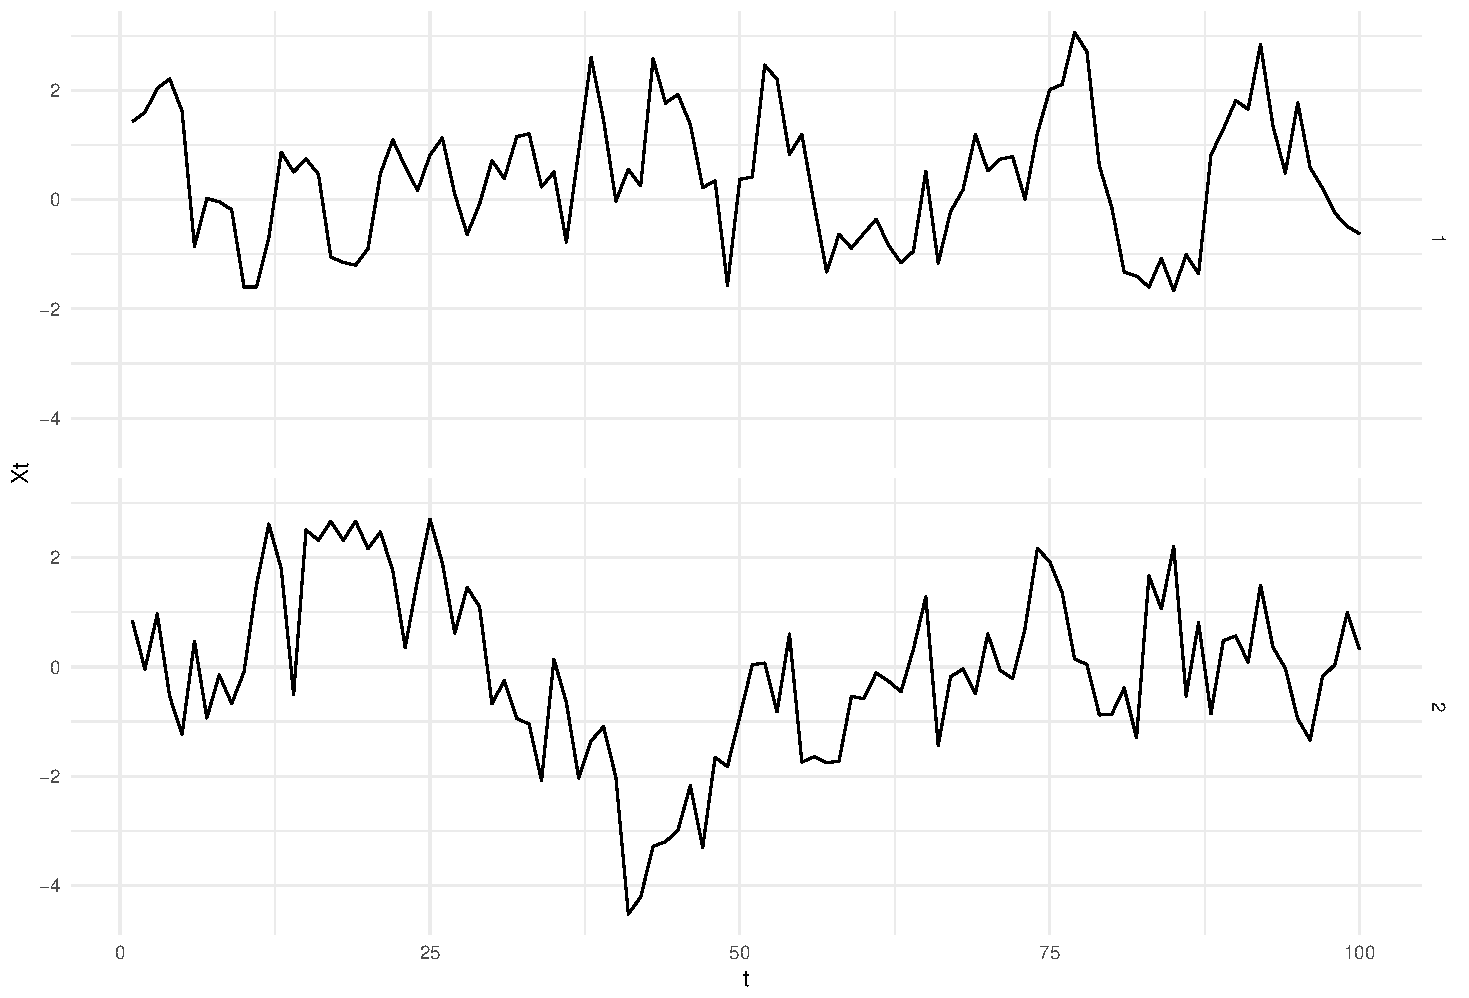
\includegraphics[scale=0.4]{ar_paths.pdf}
  \caption{Top panel: AR(1), bottom panel: AR(2)}
  \end{figure}
\end{frame}


\begin{frame}
\frametitle{Goodness of fit test}
Perhaps the most commonly used goodness of fit test in time series:
\begin{block}{Ljung-Box test \cite{LBtest}}
The Ljung-Box statistic with $l$ lags is defined as
\begin{equation*}
Q^{(l)}(\widehat{r})=n(n+2)\sum_{k=1}^l(n-k)^{-1}\widehat{\mathrm{r}}(k)^2
\end{equation*}
where
\begin{equation*}
\widehat{\mathrm{r}}(k)=\dfrac{\sum_{t=k+1}^n(Y_t-\widehat{Y}_t)(Y_{t-k}-\widehat{Y}_{t-k})}{\sum_{t=1}^n(Y_t-\widehat{Y}_t)^2},\;\;\;k=1,...,m
\end{equation*}
is the autocorrelation function.
\end{block}

If the data is truly AR($p$) but we fit AR($q$), with $q < p$, the LB test is powered to detect the residual$^2$ autocorrelation.

\end{frame}

\begin{frame}
  \frametitle{With or without selection?}
  In an ideal world, the order $p$ would be chosen \textit{a priori}, and failing to reject the LB test would be evidence that the order was indeed large enough to capture the time dependence of the errors. \\

  \

  
  But we don't live in an ideal world... \\

  \ 
 
  In practice, people will use the data to choose $p$. \\
\end{frame}


\begin{frame}
\frametitle{Model estimation and model selection}
To fit an autoregressive model to the data, the parameters $\phi_t$ are usually estimated through Yule-Walker/Burg/Least-Squares procedures, and the order $p$ is chosen by minimizing the AIC/$\mathrm{AIC_C}$/BIC. For concreteness we consider the $\mathrm{AIC_C}$\\

\begin{block}{$\mathrm{AIC_C}$ statistic for an autoregressive model}
  To choose the order $p$, we use the proposal of \cite{AICC}
%  an approximately unbiased estimator of $\mathbb{E}_F[-2\log L(\widehat{\Phi}_m,\widehat{\sigma}_m^2)]$, 
\begin{equation}\label{eq:AICCCliff}
\mathrm{AIC_C}=n(\log\widehat{\sigma}_m^2+1)+\dfrac{2n(m+1)}{n-m-2}.
\end{equation}
where $\widehat{\sigma}_m^2$ can be obtained by the Yule-Walker method, or some other asymptotically equivalent method.
\end{block}
\end{frame}



\begin{frame}
\frametitle{An example: AR(3)}
Suppose our true model is an AR(3) process: 
\begin{equation*}
Y_{t+1}=\phi_1Y_{t}+\phi_2Y_{t-1}+\phi_3Y_{t-2}+\varepsilon_{t+1}, \;\;\text{for }t\ge3,
\end{equation*}
where $\varepsilon_{t+1}\sim\mathcal{N}(0,\sigma_3^2)$. In our example, 
\begin{equation*}
\phi_1 = -0.33, \phi_2 = -0.17, \phi_3 = -0.12.
\end{equation*}
If we choose the order 3 then estimate the model as AR(3),
\begin{equation*}
Y_{t+1}=\widehat{\phi}_{31}Y_{t}+\widehat{\phi}_{32}Y_{t-1}+\widehat{\phi}_{33}Y_{t-2}
\end{equation*}
with estimated variance $\widehat{\sigma}_3^2$. If we choose the order 2, then
\begin{align*}
Y_{t+1}=\widehat{\phi}_{21}Y_{t}+\widehat{\phi}_{22}Y_{t-1}
\end{align*}
with estimated variance $\widehat{\sigma}_2^2$, or the order 1 and as AR(1)
\begin{align*}
Y_{t+1}=\widehat{\phi}_{11}Y_{t}
\end{align*}
with estimated variance $\widehat{\sigma}_1^2$.
\end{frame}

\begin{frame}
  \frametitle{A selection event example}
By the $\mathrm{AIC_C}$ statistic defined in (\ref{eq:AICCCliff}), order 2 is chosen if and only if
\begin{equation*}
\mathrm{AIC_{C}}(3)>\mathrm{AIC_{C}}(2)<\mathrm{AIC_{C}}(1)\Leftrightarrow c_{3} \widehat{\sigma}_3^2> c_2 \widehat{\sigma}_2^2 <  c_{1} \widehat{\sigma_{1}^2}
\end{equation*}
where $c_p$ are constants. \\

\

We now show simulated distributions of the LB test statistic under different selection events in the following figures, first without selection and then with selection. \\

\

Remember, we reject for large values of the LB statistic.
\end{frame}


\begin{frame}
\frametitle{Observed LB vs null distribution, without selection}
\begin{figure}
\begin{center}
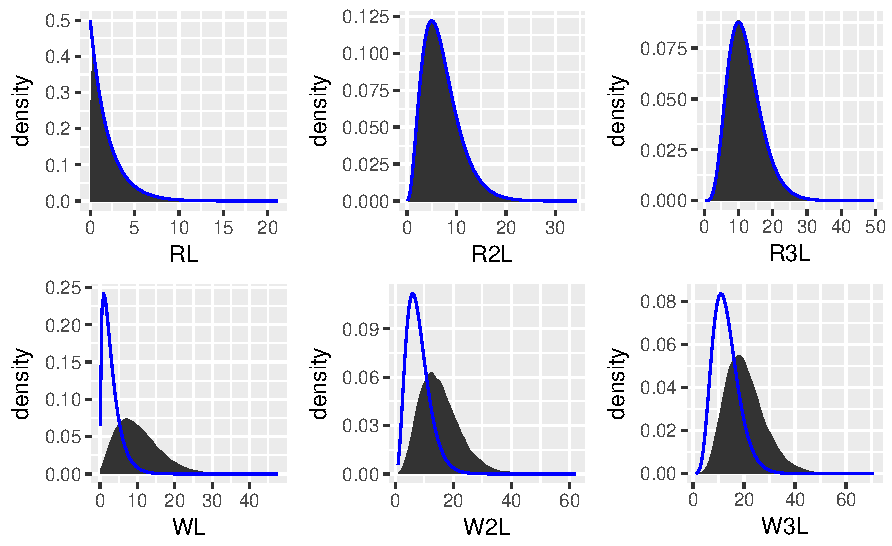
\includegraphics[scale=0.6]{true3fit2_all}
\caption{Truth is AR(3). Top row: fitted with $p = 3$. Bottom row: fitted with $p = 2$. Distributions shown for LB with lags 5, 10, 15.}
\end{center}
\end{figure}
\end{frame}


\begin{frame}
\frametitle{Observed LB vs null distribution, with selection}
\begin{figure}[H]
\begin{center}
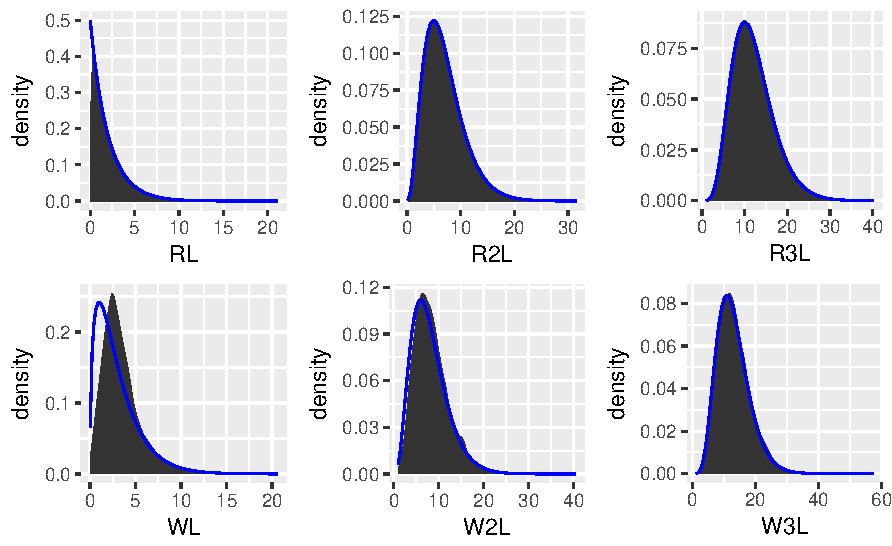
\includegraphics[scale=0.6]{true3fit2_selected}
\caption{Truth is AR(3). Top row: when $\mathrm{AIC_C}$ selects $p = 3$. Bottom row: when $p = 2$ is selected. Distributions shown for LB with lags 5, 10, 15.}
\end{center}
\end{figure}
\end{frame}



%% \begin{frame}
%% \frametitle{An example: AR(3) -- When the wrong order is chosen II}
%% By the $\mathrm{AIC_C}$ statistic defined in (\ref{eq:AICCCliff}), if order 1 is chosen and AR(1) is fitted, the selection would be made from \begin{equation*}
%% \mathrm{AIC_{C}}(3)>\mathrm{AIC_{C}}(1)\Leftrightarrow e^\frac{4(n-1)}{(n-3)(n-5)}\widehat{\sigma}_3^2>\widehat{\sigma}_1^2.
%% \end{equation*}
%% The distribution of the test statistics given the event selected is given in the following figures.
%% \end{frame}

%% \begin{frame}
%% \frametitle{An example: AR(3) -- When the wrong order is chosen II}
%% \begin{figure}
%% \begin{center}
%% 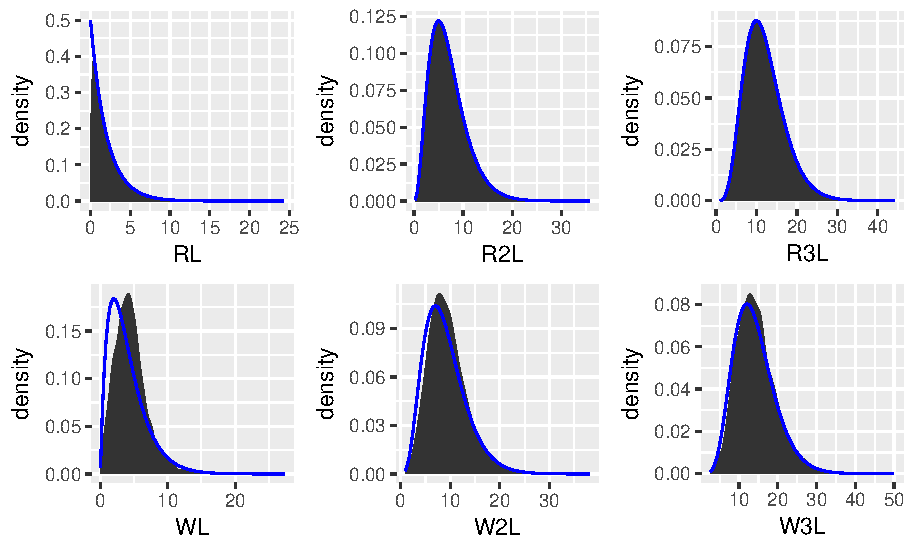
\includegraphics[scale=0.6]{true3fit1_selected}
%% \caption{With selection, true order is 3, fitted order is 1. Lag $l=5$ is examined. Black: the first row, distribution of the test statistics at lag $l/2l/3l$ when the right order is selected; the second row, the wrong order selected. Blue: the first row, distribution of $\chi^2$ with degree of freedom $l/2l/3l-3$; the second row, $\chi^2$ with df $l/2l/3l-1$.}
%% \end{center}
%% \end{figure}
%% \end{frame}
%% \begin{frame}
%% \frametitle{An example: AR(3) -- When the wrong order is chosen II}
%% \begin{figure}
%% \begin{center}
%% 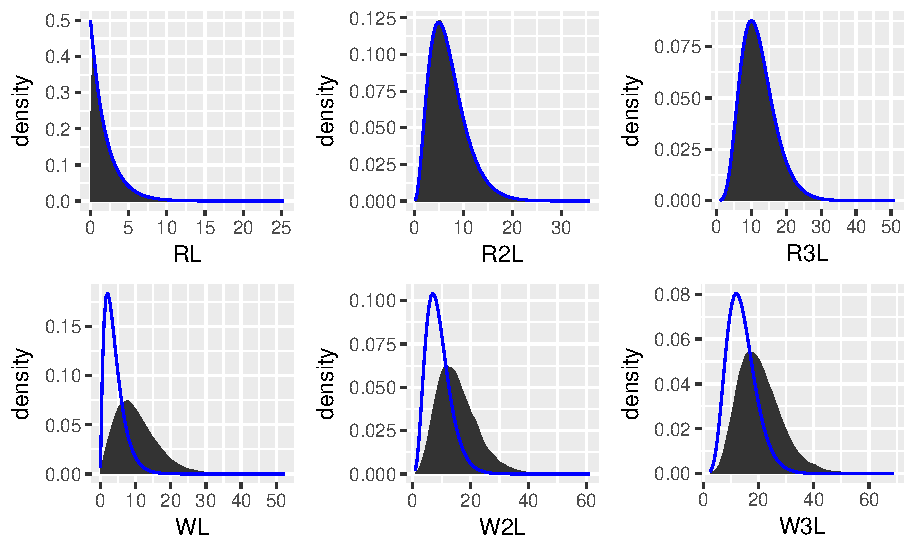
\includegraphics[scale=0.6]{true3fit1_all}
%% \caption{With selection, true order is 3, fitted order is 1. Lag $l=5$ is examined. Black: the distribution of all events. Blue: the first row, distribution of $\chi^2$ with degree of freedom $l/2l/3l-3$; the second row, $\chi^2$ with df $l/2l/3l-1$.}
%% \end{center}
%% \end{figure}
%% \end{frame}

\begin{frame}
\frametitle{No power conditional on selecting wrong order!}


\begin{itemize}
\item When we fit the right model (R, top row) the test statistic matches its null distribution
\item When we fit the wrong model \textit{deterministically} (W, 2nd row, 1st fig) the test statistic is stochastically larger, indicating power to reject
\item But when we fit the wrong model \textit{by selection} (W, 2nd row, 2nd fig) the test statistic approximately matches its null distribution. The test is (nearly) no better than an $\alpha$-coin toss at telling us the chosen model is incorrect
\end{itemize}
\end{frame}




\section{Linear regression}
\subsection{F-tests of unselected variables}

\begin{frame}
\frametitle{Regression example: F-tests (of unselected variables)}

\begin{itemize}
\item Regression models $E[Y] = X_A \beta_A$ for some subset $A$ of columns of a matrix $X$.
\item With nested subsets $A \subsetneq A'$, we'll conduct an $F$-test and consider this as a goodness-of-fit test for the model with variables $A$.
\item In \texttt{R} we just use the \texttt{anova} function with these two linear models.
\end{itemize}

The distribution of the $F$-statistic is derived, of course, under the assumption that $A$ and $A'$ have been chosen \textit{a priori}... \\

\ 

(An idea similar to this is mentioned in \cite{tian2015selective})
\end{frame}


\begin{frame}
\frametitle{Regression variable selection}

\begin{itemize}
\item For concreteness, consider selecting variables using forward stepwise with BIC, i.e. in \texttt{R} with \texttt{step(..., k = log(n))}.
\item Simulation with $n = 100$ observations of $p = 10$ variables, the first two coefficients are larger than the next 3, and the last 5 are all 0.
\item In this low-dimensional example, we'll take $A' = \{ 1, \ldots, 10 \}$ for simplicity.
\item We'll consider the $F$-test (1) with $A$ chosen deterministically as the first 2 variables, and (2) with $A$ selected by forward stepwise.
\end{itemize}
\end{frame}

\begin{frame}
  \frametitle{Profile of model selection events}
  \centering
  \begin{figure}
  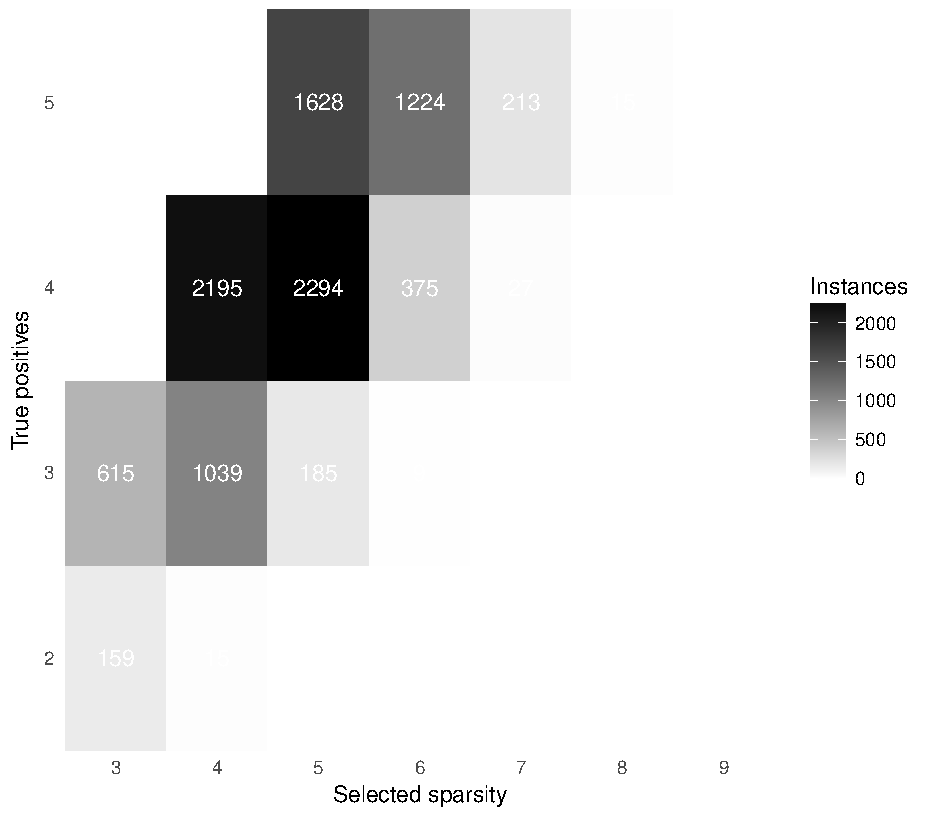
\includegraphics[scale=0.45]{fstepbic2.pdf}
  \end{figure}
\end{frame}



\begin{frame}
  \frametitle{Distributions of $p$-values for full-model $F$-tests}
  \centering
  \begin{figure}
  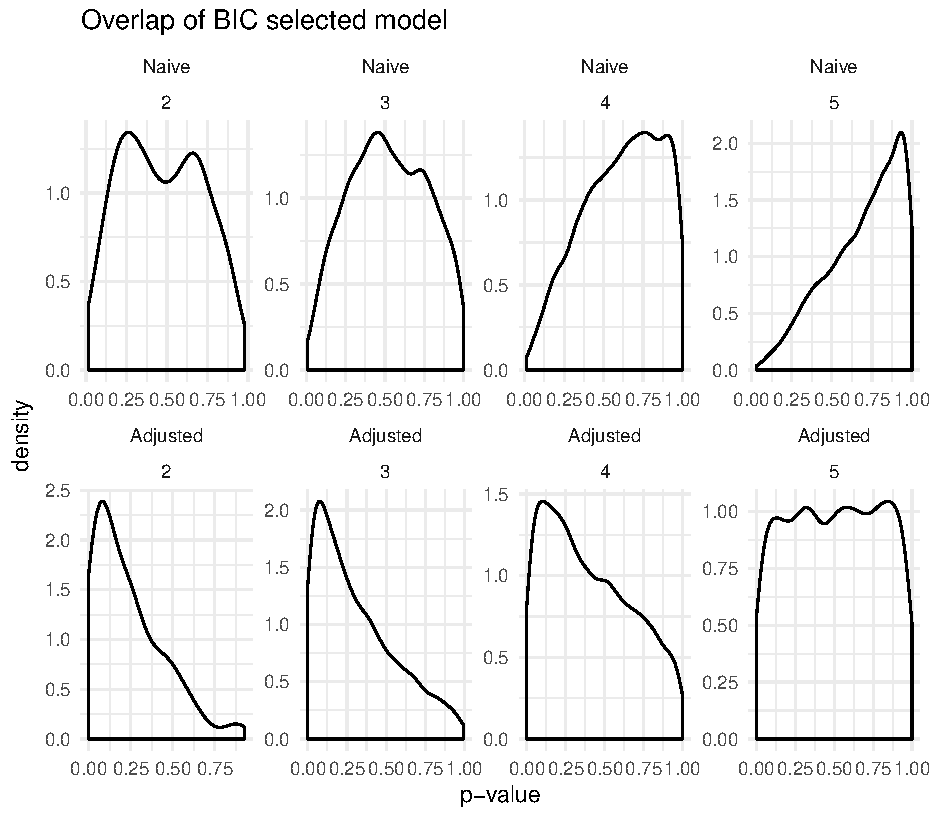
\includegraphics[scale=0.5]{fdists_both2}
  \caption{Top: unadjusted $p$-values. Bottom: adjusted for selection.}
  \end{figure}
\end{frame}


\begin{frame}
  \frametitle{Probability of rejection}


\begin{table}

\caption{\label{tab:1}Probability of rejection at level 0.1, conditional on size of overlap}
\centering
\begin{tabular}[t]{l|r|r}
\hline
pvalue & overlap & Pr(reject)\\
\hline
Naive & 2 & 0.056\\
\hline
Naive & 3 & 0.032\\
\hline
Naive & 4 & 0.017\\
\hline
Naive & 5 & 0.005\\
\hline
Adjusted & 2 & 0.328\\
\hline
Adjusted & 3 & 0.251\\
\hline
Adjusted & 4 & 0.156\\
\hline
Adjusted & 5 & 0.101\\
\hline
\end{tabular}
\end{table}

  
\end{frame}



\begin{frame}
  \frametitle{Power conditional on not selecting all true positives}


\begin{table}

\caption{\label{tab:}Probability of rejection at level 0.1, conditional on overlap less than 5}
\centering
\begin{tabular}[t]{l|r}
\hline
pvalue & Pr(reject)\\
\hline
Naive & 0.022\\
\hline
Adjusted & 0.186\\
\hline
\end{tabular}
\end{table}

  
\end{frame}


\subsection{Orthogonal case / many means}

\begin{frame}
\frametitle{Many means example (with new math?)}

\begin{itemize}
\item Independent $Z_i \sim \mathcal N(\mu_i, 1)$, $i = 1, \ldots, p$.
\item Apply hard-thresholding: discard any $Z_i$ with $|Z_i| < C$.
\item Goodness-of-fit test: $\chi^2$ with discarded effects
\end{itemize}

\begin{block}{Test statistic}
  Suppose $Z_1, \ldots, Z_m$ are discarded, i.e. they are less than $C$ in absolute value. We will use
  \begin{equation*}
    T = \sum_{i=1}^m Z_i^2
  \end{equation*}
  as a test statistic.
\end{block}

Not distributed as $\chi^2$ --  each term in the sum is truncated.

\end{frame}

\begin{frame}
  \frametitle{The $m=2$ case}

\begin{block}{Distribution of a sum of truncated $\chi^2_1$ random variables}
Suppose $Z_i \sim \mathcal N(0, 1) \mid_{[-C, C]}$, then the density function $f(z)$ of $Z_1^2+Z_2^2$ is

\begin{equation*}
 [1 - 2\Phi(-C)]^2 f(z) = 
\begin{cases}
  \dfrac{1}{2}e^{-y/2} & 0 \leq z \leq C^2 \\
  \dfrac{1}{\pi}e^{-y/2}\left[2\arcsin\left(\dfrac{c}{\sqrt{y}}\right)-\dfrac{\pi}{2}\right] & C^2 < z \leq 2C^2 \\
  0 & \text{ otherwise}\\
\end{cases}
\end{equation*}
\end{block}

When $m > 2$ calculations get nastier (but for large $m$ could use asymptotic results)

\end{frame}

\begin{frame}
\frametitle{When $m=2$}
\begin{figure}
\begin{center}
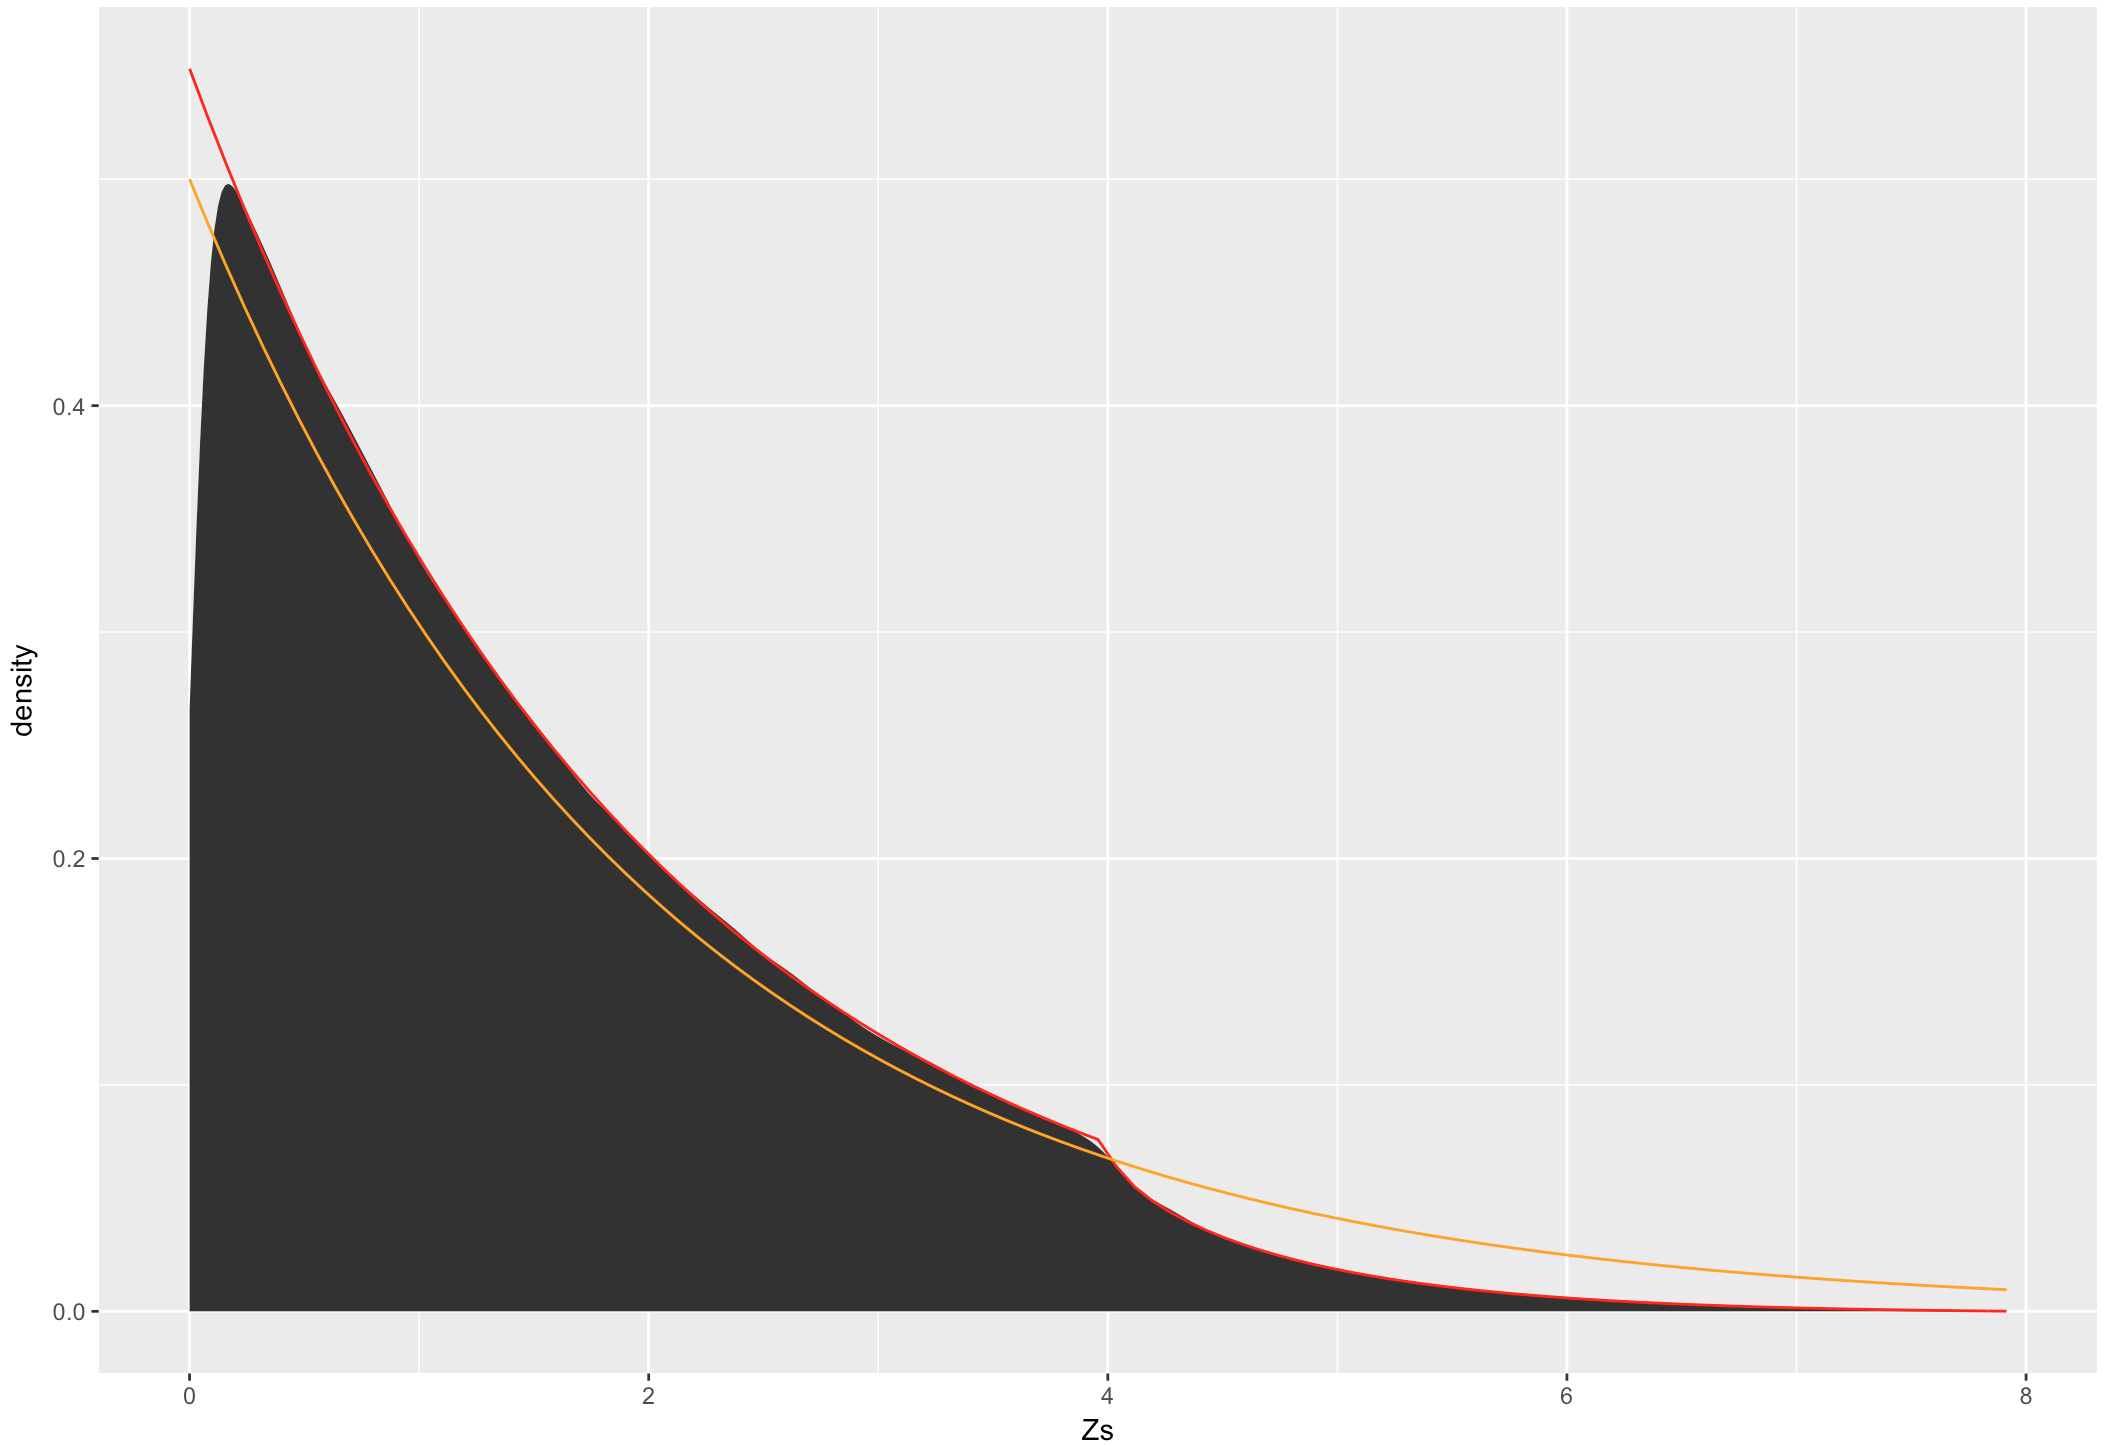
\includegraphics[scale=0.3]{m2.png}
\end{center}
\end{figure}
\end{frame}


\begin{frame}
\frametitle{Conditional power in the $m = 1$ case}

\begin{figure}
\begin{center}
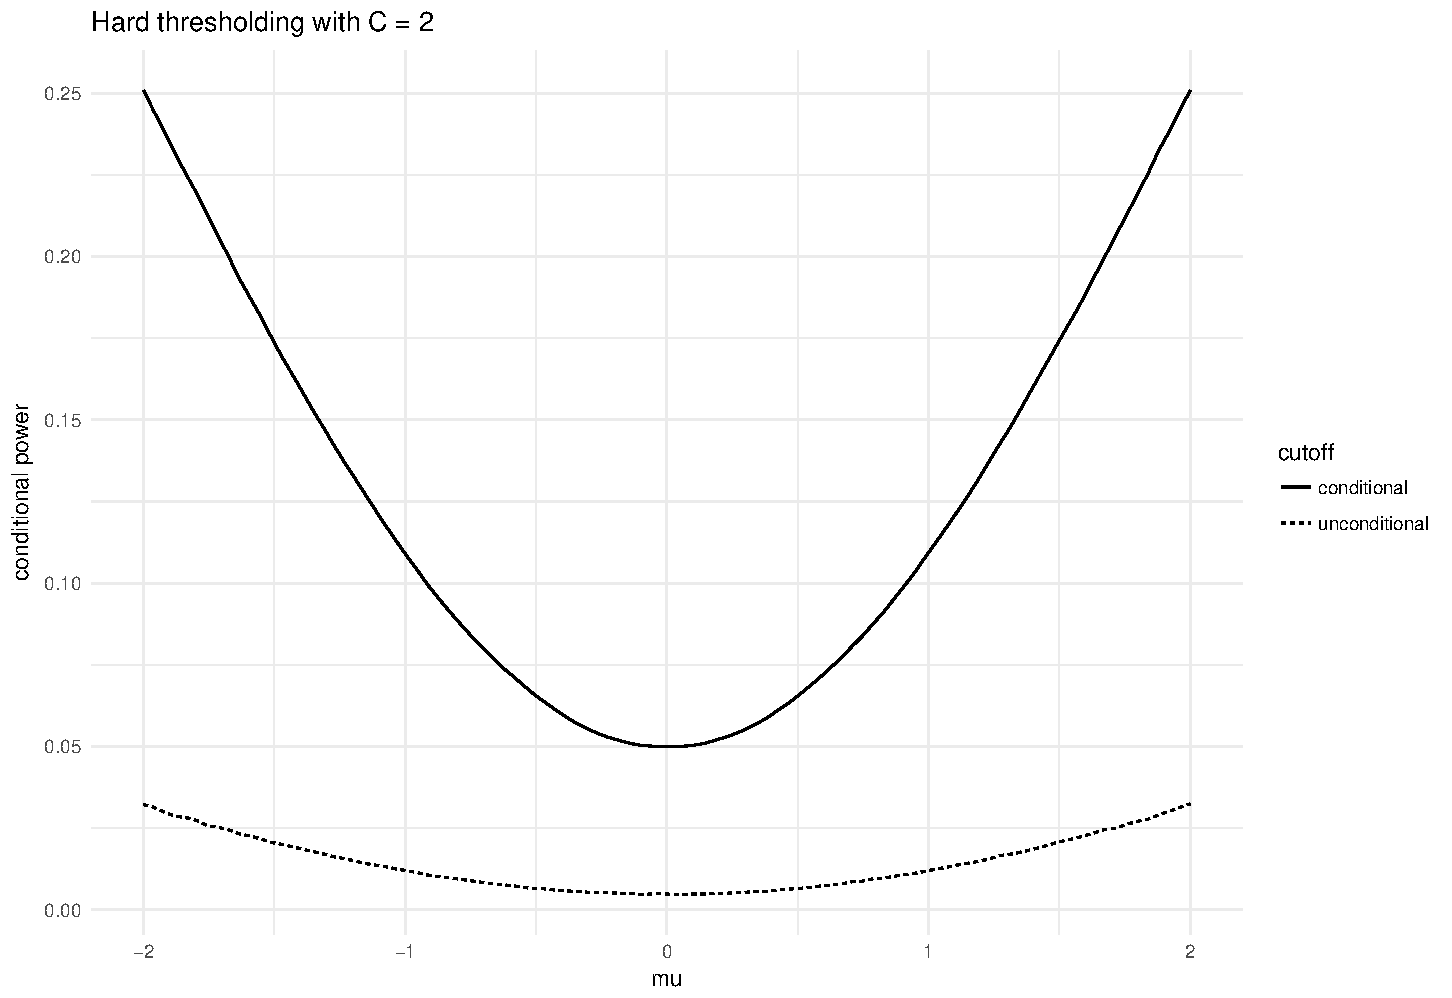
\includegraphics[scale=0.45]{powerm1.pdf}
\end{center}
\end{figure}

\end{frame}


%% \begin{frame}
%% \frametitle{When $m=3$}

%% After we apply convolution, the density function of $z_1^2+z_2^2+z_3^2$ would be 
%% \begin{equation*}
%% f_{z_1^2+z_2^2+z_3^2}(y)=\int_{-\infty}^\infty f_{z_3^2}(y-u)f_{z_1^2+z_2^2}(u)du.
%% \end{equation*}
%% Note that, the common support becomes
%% \begin{equation*}
%% \begin{cases}
%% 0\le y-u\le C^2\\
%% 0\le u\le 2C^2
%% \end{cases}
%% \Leftrightarrow\;\;\;\;\;
%% \begin{cases}
%% y-C^2\le u\le y\\
%% 0\le u\le 2C^2
%% \end{cases}.
%% \end{equation*}
%% \end{frame}

%% \begin{frame}
%% \frametitle{When $m=3$}
%% \begin{block}{Density function of $z_1^2+z_2^2+z_3^2$}
%% \begin{equation*}
%% f_{z_1^2+z_2^2+z_3^2}(y)=\int_{-\infty}^\infty f_{z_3^2}(y-u)f_{z_1^2+z_2^2}(u)du
%% \end{equation*}
%% \end{block}
%% \begin{itemize}
%% \item When $y\le C^2$, $z_1^2+z_2^2+z_3^2$ is distributed as $\chi_3^2$\\
%% \begin{equation*}
%% f_{z_1^2+z_2^2+z_3^2}(y)=\int_0^yf_{z_3^2}(y-u)f_{z_1^2+z_2^2}(u)du=\dfrac{1}{\sqrt{2\pi}}\sqrt{y}e^{-y/2}.
%% \end{equation*}
%% \item When $y\in[C^2,2C^2)$, the support for $u$ is from $y-C^2$ to $y$,
%% \begin{equation*}
%% f_{z_1^2+z_2^2+z_3^2}(y)=\dfrac{1}{\sqrt{2\pi}}e^{-2/y}\left(3C-2\sqrt{y}\right).
%% \end{equation*}
%% \end{itemize}
%% \end{frame}
%% \begin{frame}
%% \frametitle{When $m=3$}
%% \begin{block}{Density function of $z_1^2+z_2^2+z_3^2$}
%% \begin{equation*}
%% f_{z_1^2+z_2^2+z_3^2}(y)=\int_{-\infty}^\infty f_{z_3^2}(y-u)f_{z_1^2+z_2^2}(u)du
%% \end{equation*}
%% \end{block}
%% \begin{itemize}
%% \item When $y \in [2C^2,3C^2)$, the support for $u$ is from $y-C^2$ to $2C^2$,
%% \begin{align}\label{eq:lauren}
%% f_{z_1^2+z_2^2+z_3^2}(y)=&\dfrac{1}{\pi\sqrt{2\pi}}e^{-2/y} \nonumber\\
%% &\cdot\left[2i\sqrt{y}\log\dfrac{(C^2-i\sqrt{y(y-2C^2)})(C^2-y)}{C^4+2C^2\left(i\sqrt{y(y-2C^2)}+y\right)-y^2}\right]
%% \end{align}
%% \end{itemize}
%% \end{frame}
%% \begin{frame}
%% \frametitle{When $m=3$}
%% \begin{itemize}
%% \item[] \begin{align*}
%% +&\dfrac{2\sqrt{2}C}{\pi\sqrt{\pi}}e^{-2/y}\left[\arctan\left(\dfrac{3C^2-y}{2C\sqrt{y-2C^2}}\right)+\arctan\left(\dfrac{C}{\sqrt{y-2C^2}}\right)\right]\\
%% -&\dfrac{C}{\sqrt{2\pi}}e^{-2/y},
%% \end{align*}
%% where we could apply Laurent series expansion at $y=\infty$ on part (\ref{eq:lauren}). 
%% \item When $y \in [3C^2,\infty)$, out of the common support,
%% \begin{equation*}
%% f_{z_1^2+z_2^2+z_3^2}(y)=0.
%% \end{equation*}
%% \end{itemize}
%% \end{frame}

%% \begin{frame}
%% \frametitle{When $m=3$}
%% \begin{figure}
%% \begin{center}
%% 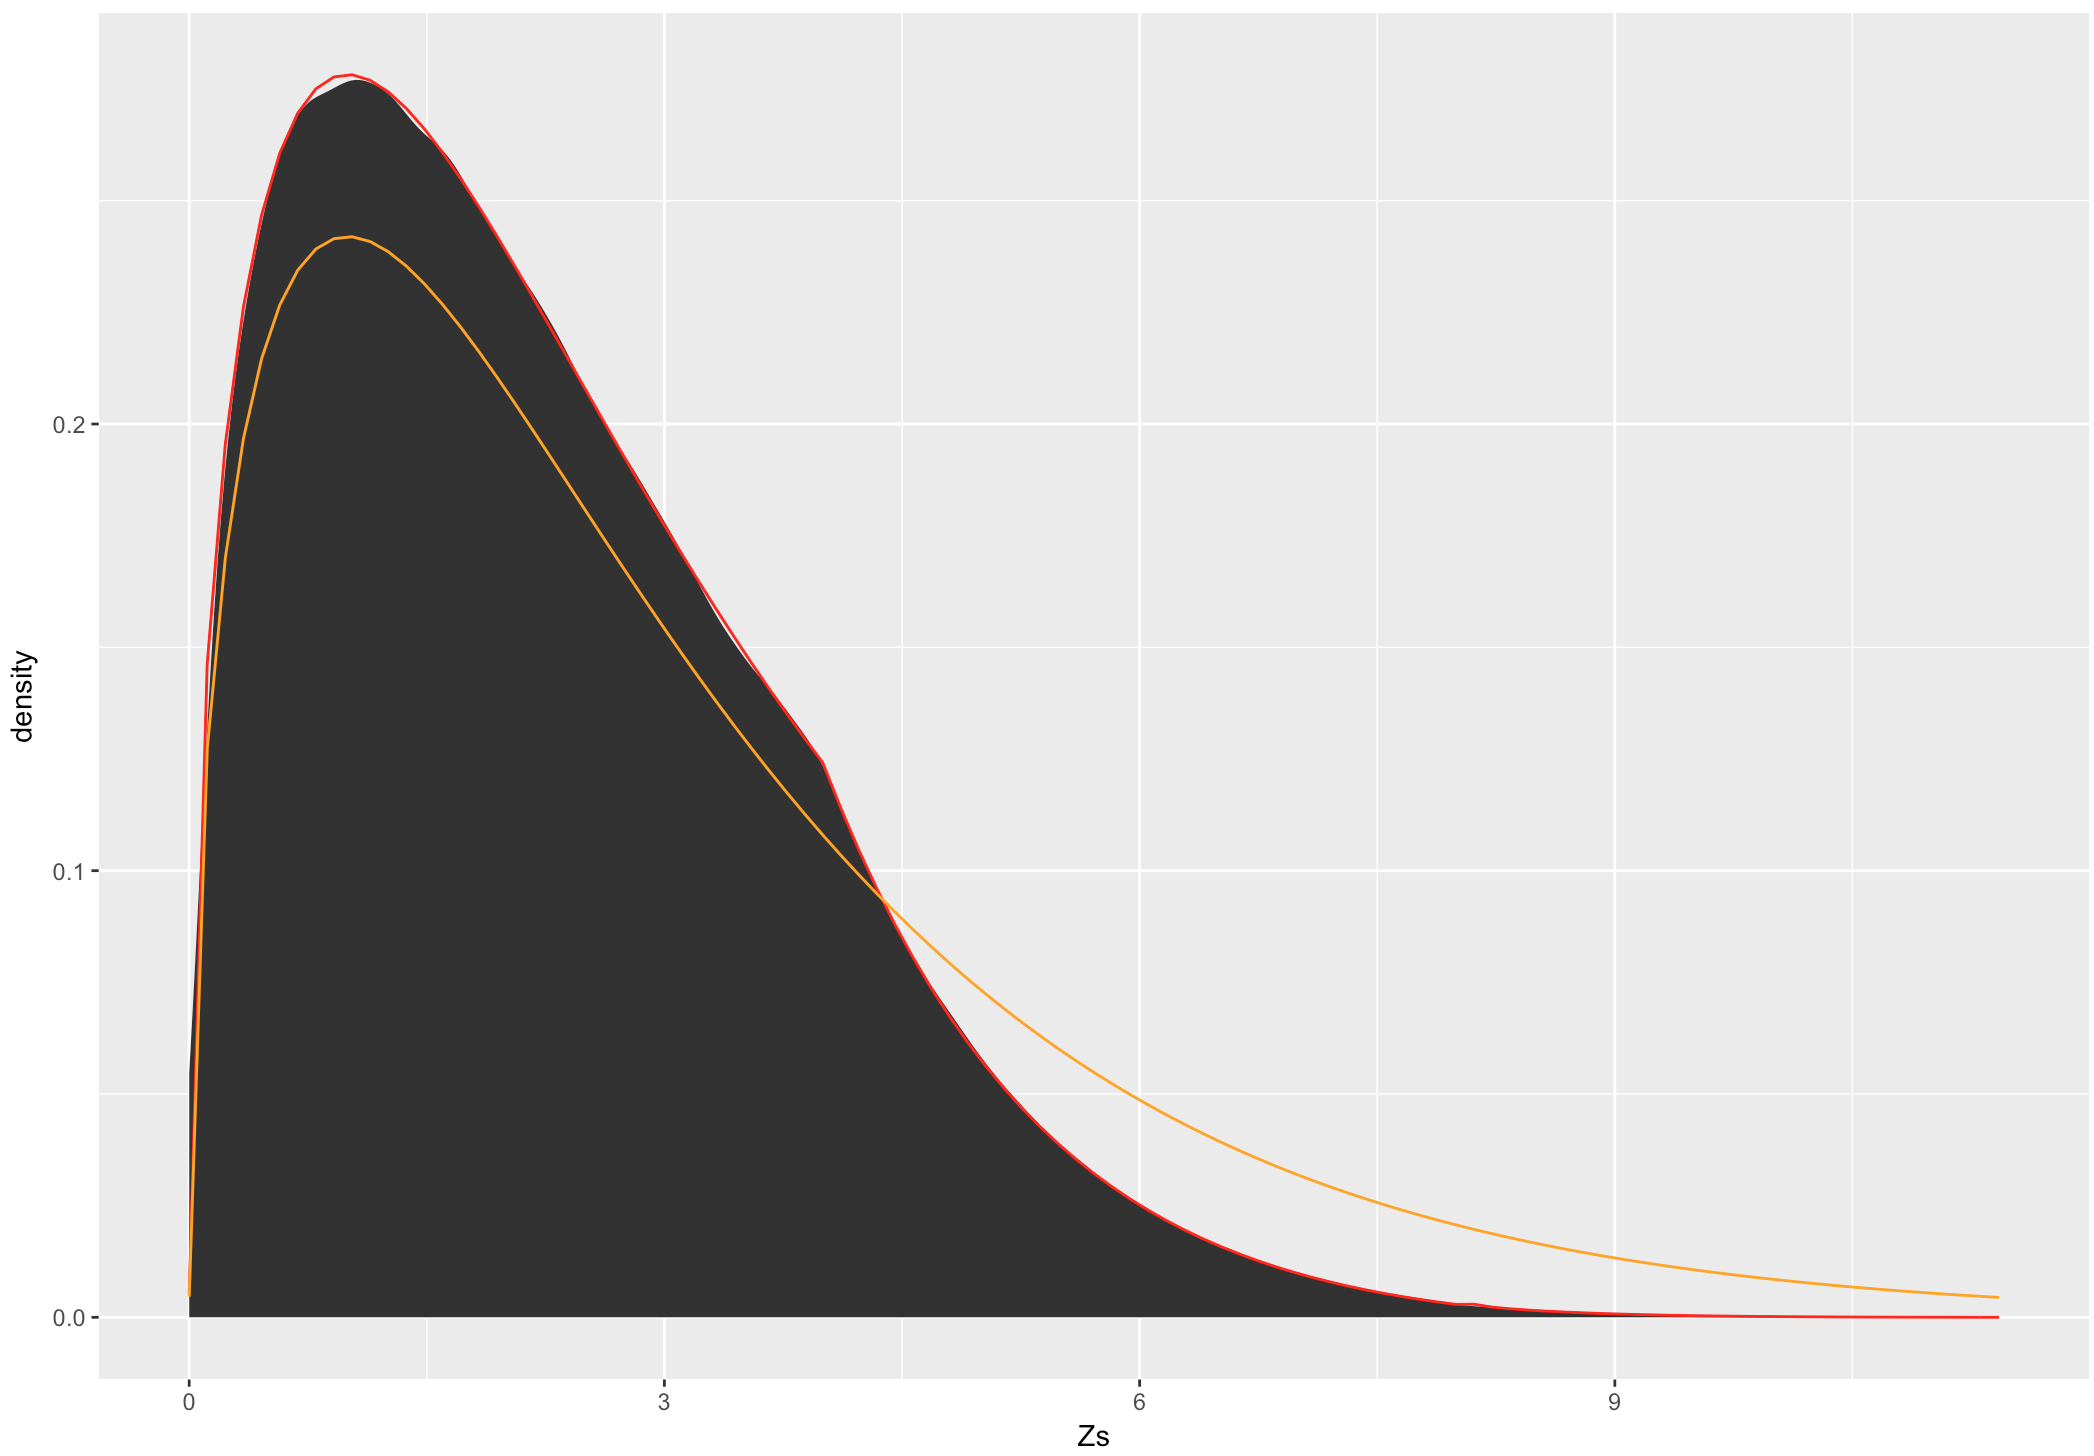
\includegraphics[scale=0.3]{expansion90.png}
%% \end{center}
%% \end{figure}
%% \end{frame}



\section{Conclusion}
\subsection{The quiet scandal for goodness-of-fit tests}

\begin{frame}
  \frametitle{Quiet scandal}

  \centering
  Goodness-of-fit tests: HUH! \\

  \ 

  What are they good for? \\

  \ 

  Absolutely nothing!? \\
  
  \

  (until we fix them)
\end{frame}


\subsection{Converging on standard practices?}

\begin{frame}
\frametitle{Converging on standard practices?}
\begin{itemize}
\item Large variety of goodness-of-fit tests in all kinds of different modeling settings.
\item Non-tests: various measures and diagnostic plots -- any kind of model assessment.
\item Important message that these are \textit{all} affected by model selection bias, not just variable significance tests or prediction/classification accuracy.
\item Can we converge on a new set of standard practices?
\item Proposal: we must make these tools as easy to use as \texttt{summary()} and diagnostic \texttt{plot()}
\end{itemize}

\end{frame}


\begin{frame}{Reference}

\bibliographystyle{apalike}
\bibliography{mybib.bib}

  
%% \begin{itemize}
%% \item Clifford M. Hurvich and Chin-Ling Tsai. Regression and time series model selection in small samples. \textit{Biometrika}, 76(1): 297-307, June 1989.
%% \end{itemize}


\end{frame}
\end{document}
